\newpage
\section{Conic Projections}
\subsection{Lambert Equal Area Conic}
\begin{figure}[H]
    \centering
    \begin{minipage}{0.30\textwidth}
        \centering
        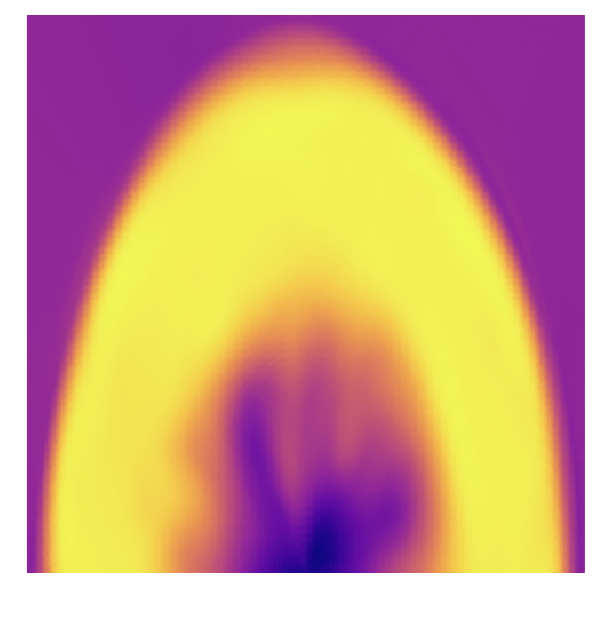
\includegraphics[width=0.9\linewidth]{figures/chapter-8/geopoth_leac.png}
        \caption{ Geopotential height raster data as Lambert Equal Area Conic projected}
        \label{fig:leac_geopoth_raster}
    \end{minipage}\hfill
    \begin{minipage}{0.30\textwidth}
        \centering
        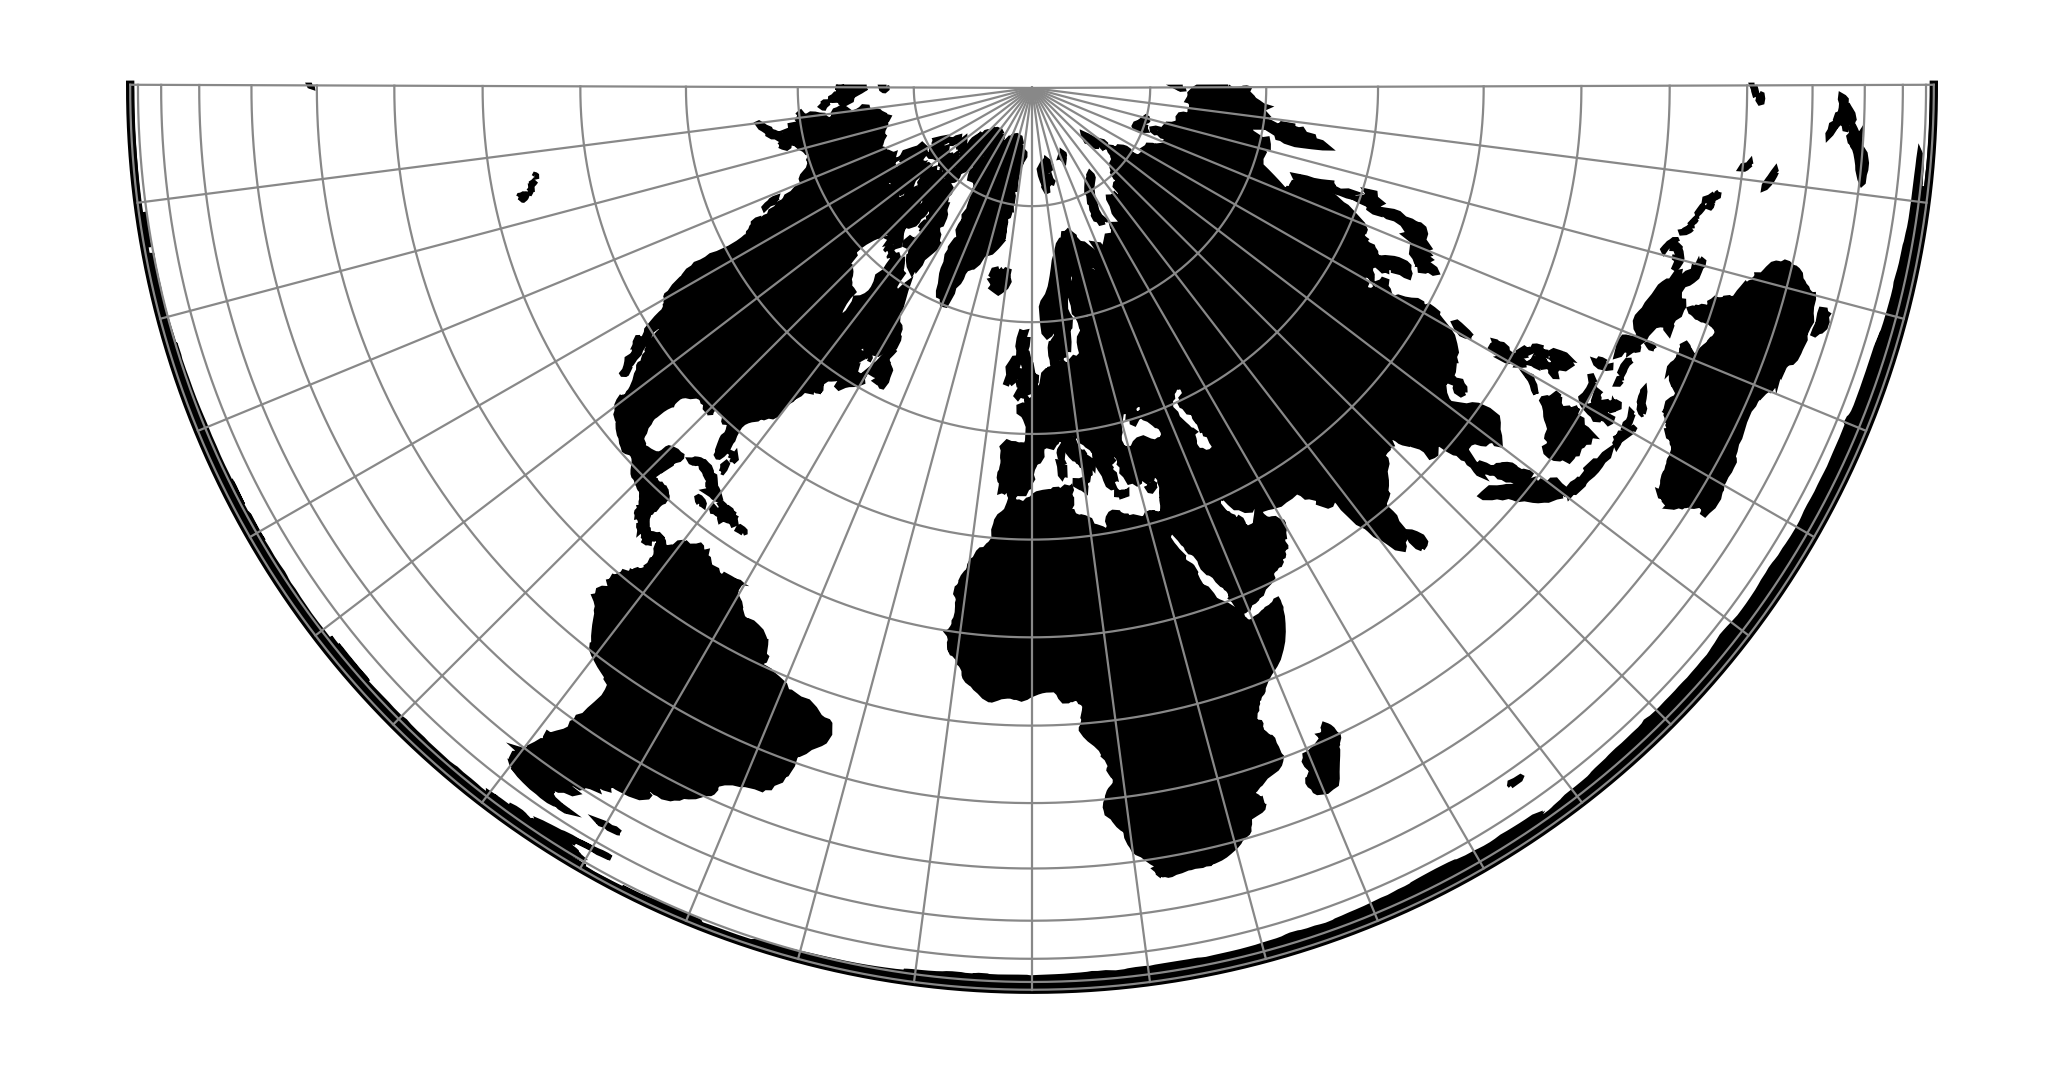
\includegraphics[width=0.9\linewidth]{figures/chapter-8/leac.png}
        \caption{Lambert Equal Area Conic (Source \cite{PROJ_SITE})}
        \label{fig:leac_proj}
    \end{minipage}\hfill
    \begin{minipage}{0.30\textwidth}
        \centering
        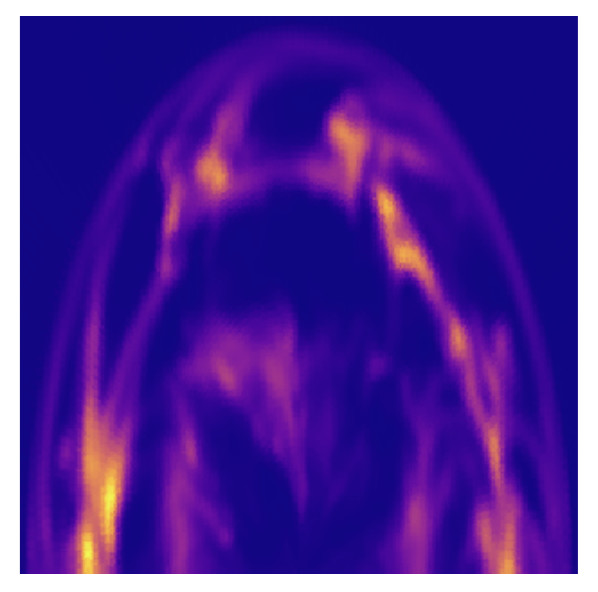
\includegraphics[width=0.9\linewidth]{figures/chapter-8/prect_leac.png}
        \caption{Precipitation raster data as Lambert Equal Area Conic projected}
        \label{fig:leac_prect_raster}
    \end{minipage}\hfill
\end{figure}
\subsection{Albers Equal Area}
\begin{figure}[h]
    \centering
    \begin{minipage}{0.30\textwidth}
        \centering
        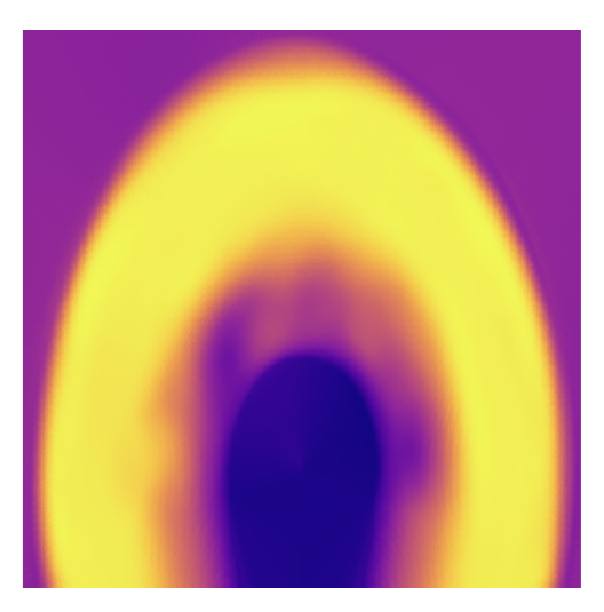
\includegraphics[width=0.9\linewidth]{figures/chapter-8/geopoth_aea.png}
        \caption{ Geopotential height raster data as Albers Equal Area projected}
        \label{fig:aea_geopoth_raster}
    \end{minipage}\hfill
    \begin{minipage}{0.30\textwidth}
        \centering
        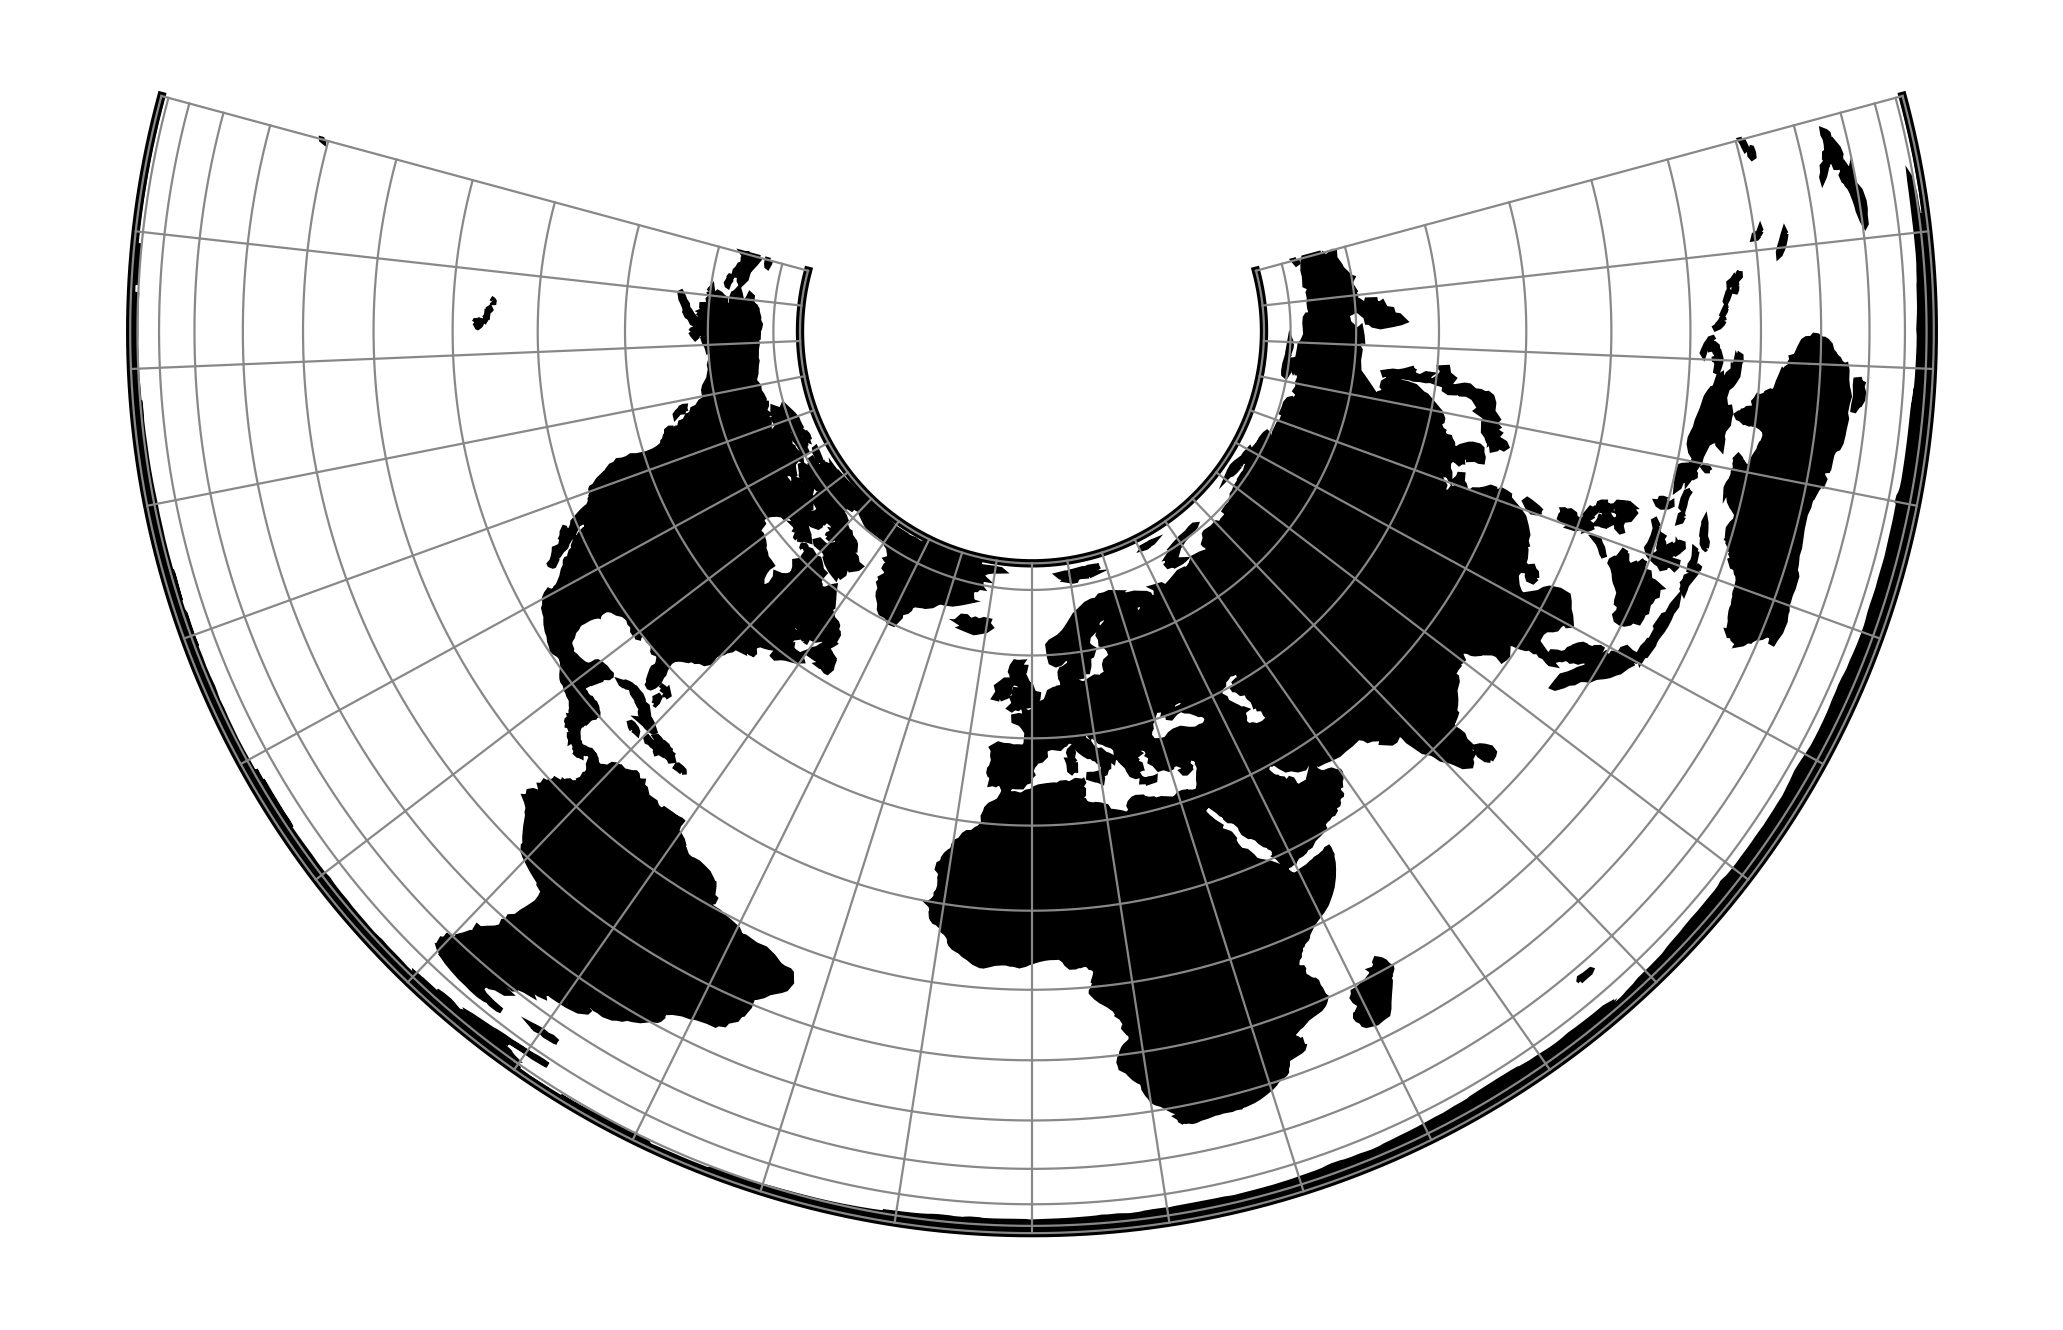
\includegraphics[width=0.9\linewidth]{figures/chapter-8/aea.png}
        \caption{Albers Equal Area (Source \cite{PROJ_SITE})}
        \label{fig:aea_proj}
    \end{minipage}\hfill
    \begin{minipage}{0.30\textwidth}
        \centering
        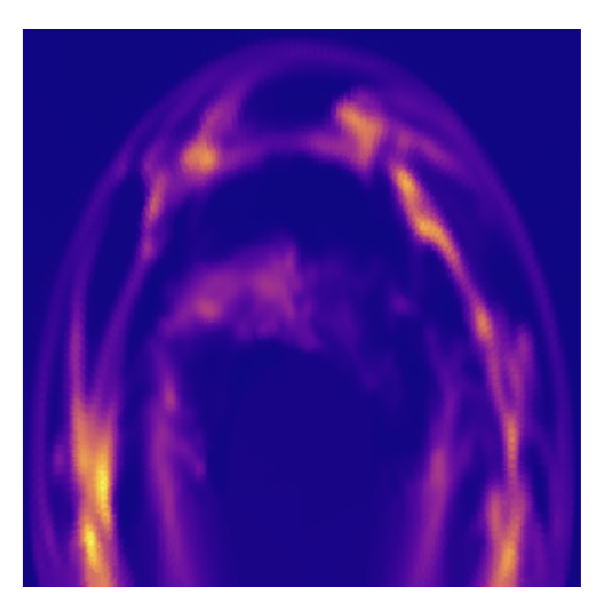
\includegraphics[width=0.9\linewidth]{figures/chapter-8/prect_aea.png}
        \caption{Precipitation raster data as Albers Equal Area projected}
        \label{fig:aea_prect_raster}
    \end{minipage}\hfill
\end{figure}
\newpage
\subsection{Vitkovsky I}
\begin{figure}[h]
    \centering
    \begin{minipage}{0.30\textwidth}
        \centering
        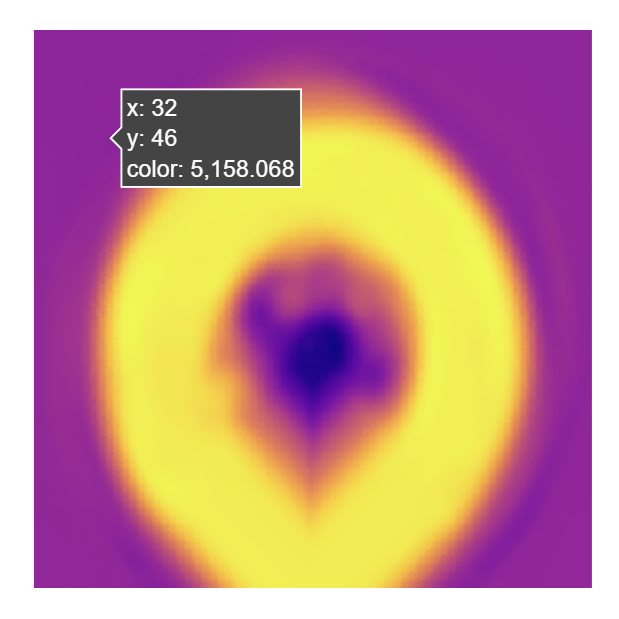
\includegraphics[width=0.9\linewidth]{figures/chapter-8/geopoth_vitk.png}
        \caption{ Geopotential height raster data as Vitkovsky I projected}
        \label{fig:vitk_geopoth_raster}
    \end{minipage}\hfill
    \begin{minipage}{0.30\textwidth}
        \centering
        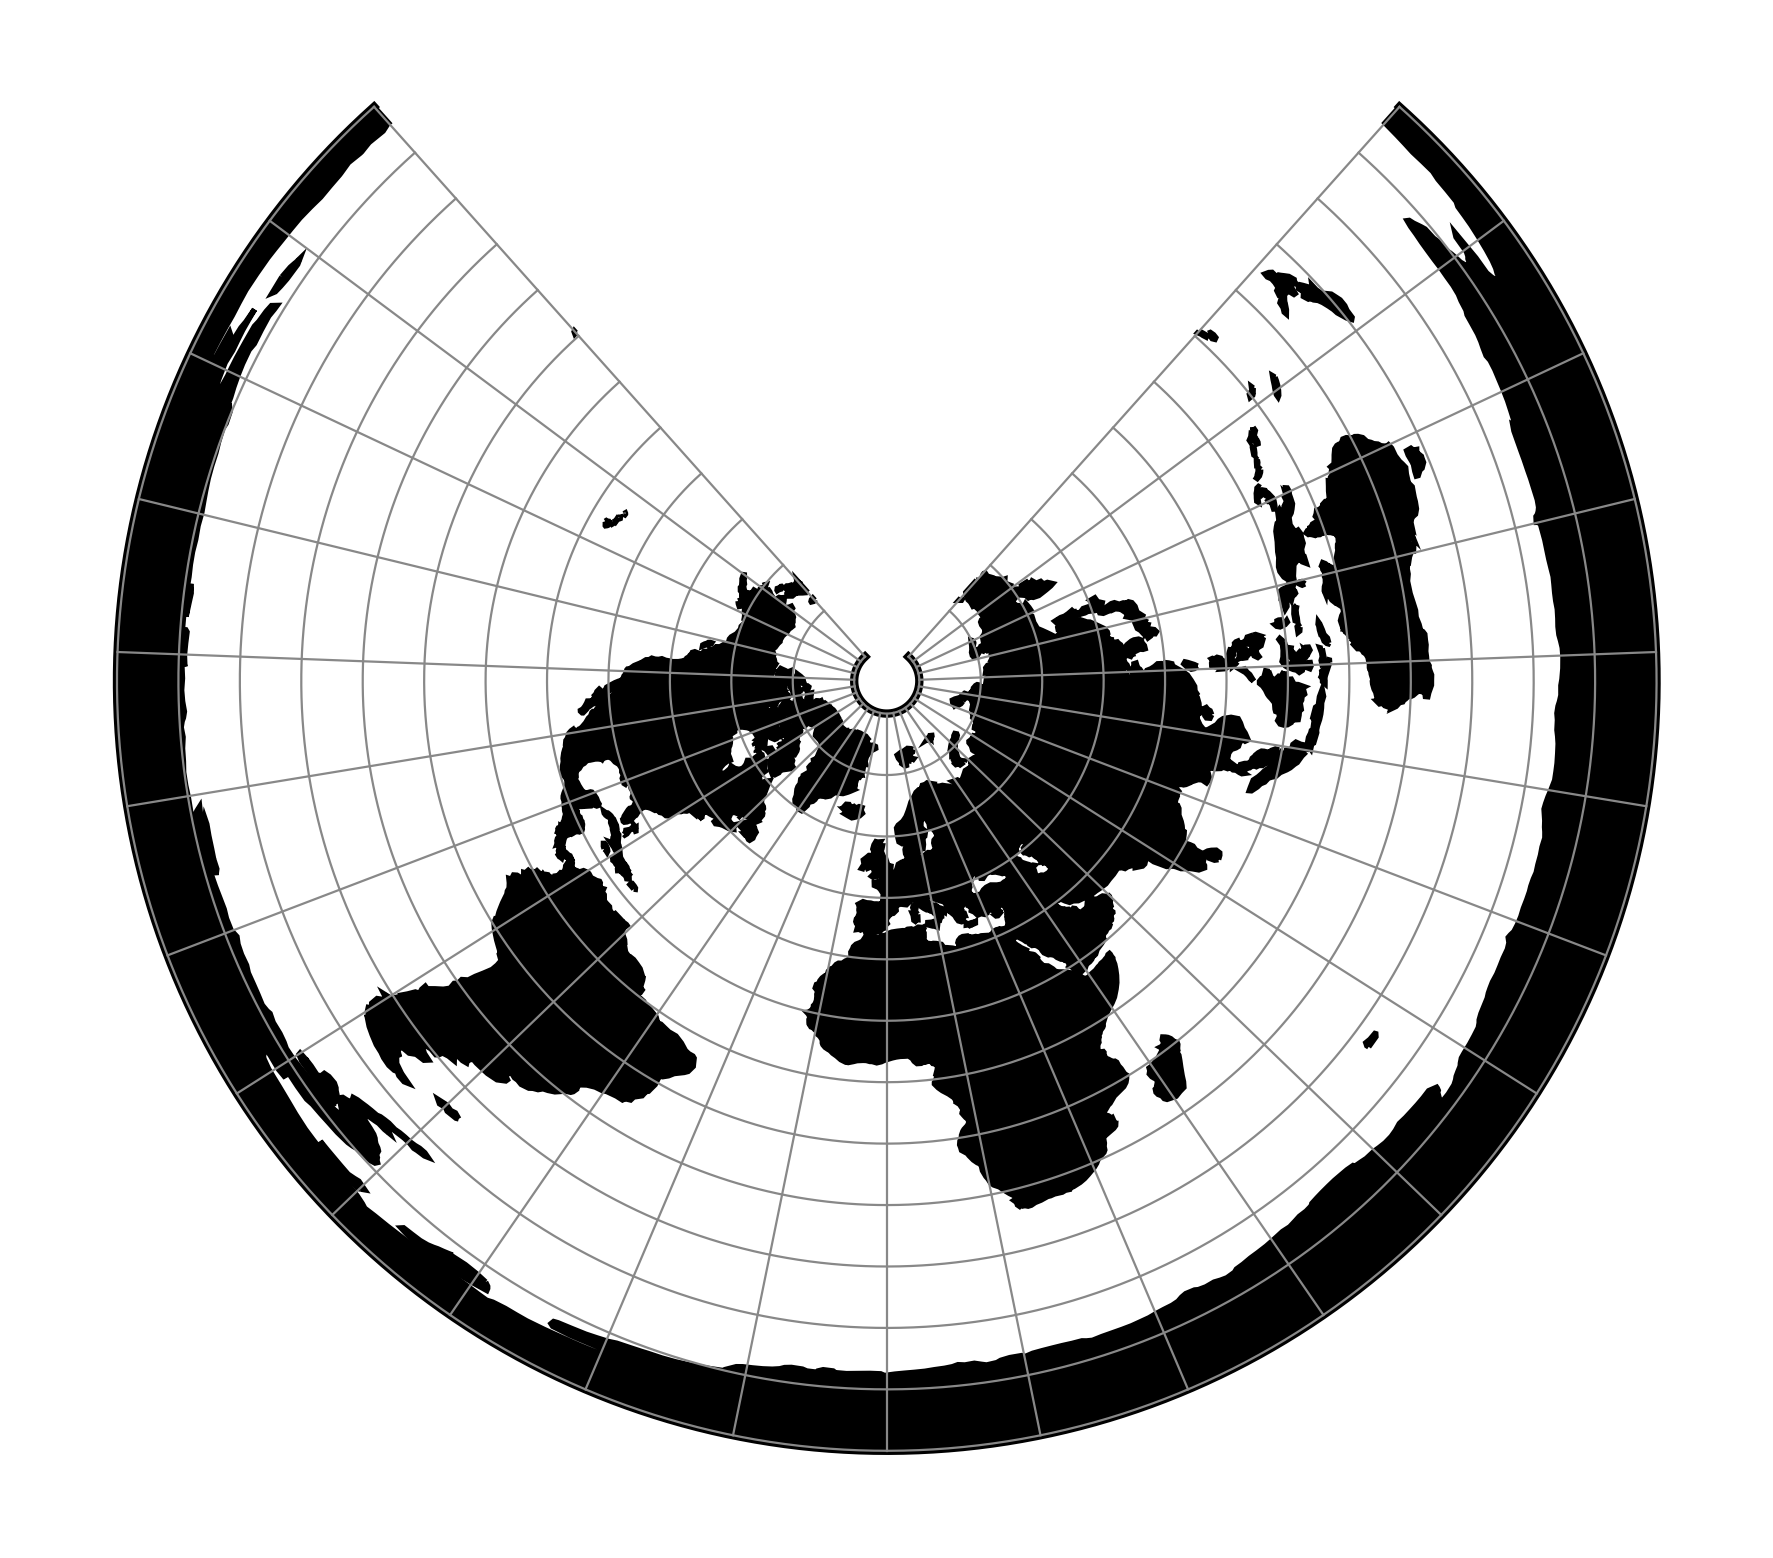
\includegraphics[width=0.9\linewidth]{figures/chapter-8/vitk1.png}
        \caption{Vitkovsky I (Source \cite{PROJ_SITE})}
        \label{fig:vitk_proj}
    \end{minipage}\hfill
    \begin{minipage}{0.30\textwidth}
        \centering
        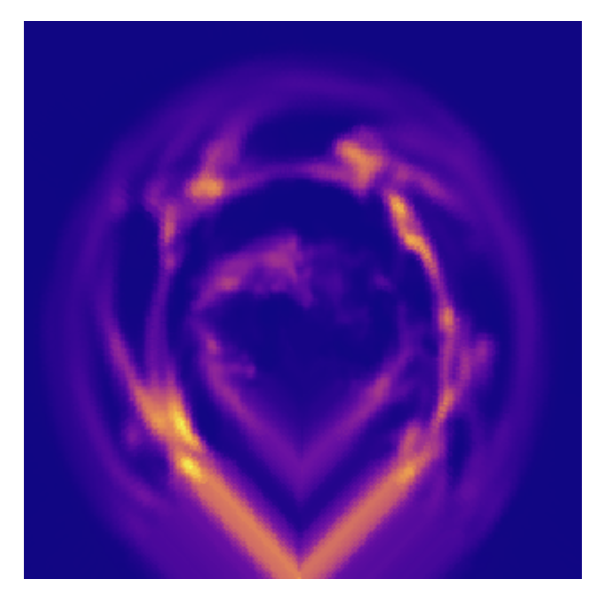
\includegraphics[width=0.9\linewidth]{figures/chapter-8/prect_vitk.png}
        \caption{Precipitation raster data as Vitkovsky I projected}
        \label{fig:vitk_prect_raster}
    \end{minipage}\hfill
\end{figure}
\subsection{Lambert Conformal Conic Alternative}
\begin{figure}[h]
    \centering
    \begin{minipage}{0.30\textwidth}
        \centering
        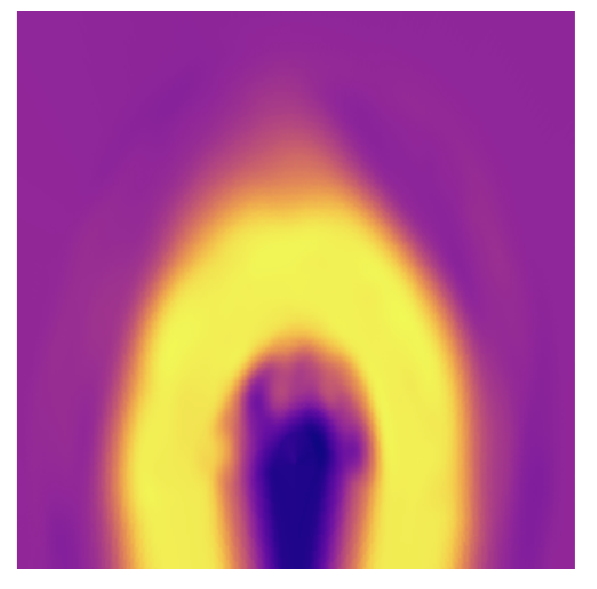
\includegraphics[width=0.9\linewidth]{figures/chapter-8/geopoth_lcca.png}
        \caption{ Geopotential height raster data as Lambert Conformal Conic Alternative projected}
        \label{fig:lcca_geopoth_raster}
    \end{minipage}\hfill
    \begin{minipage}{0.30\textwidth}
        \centering
        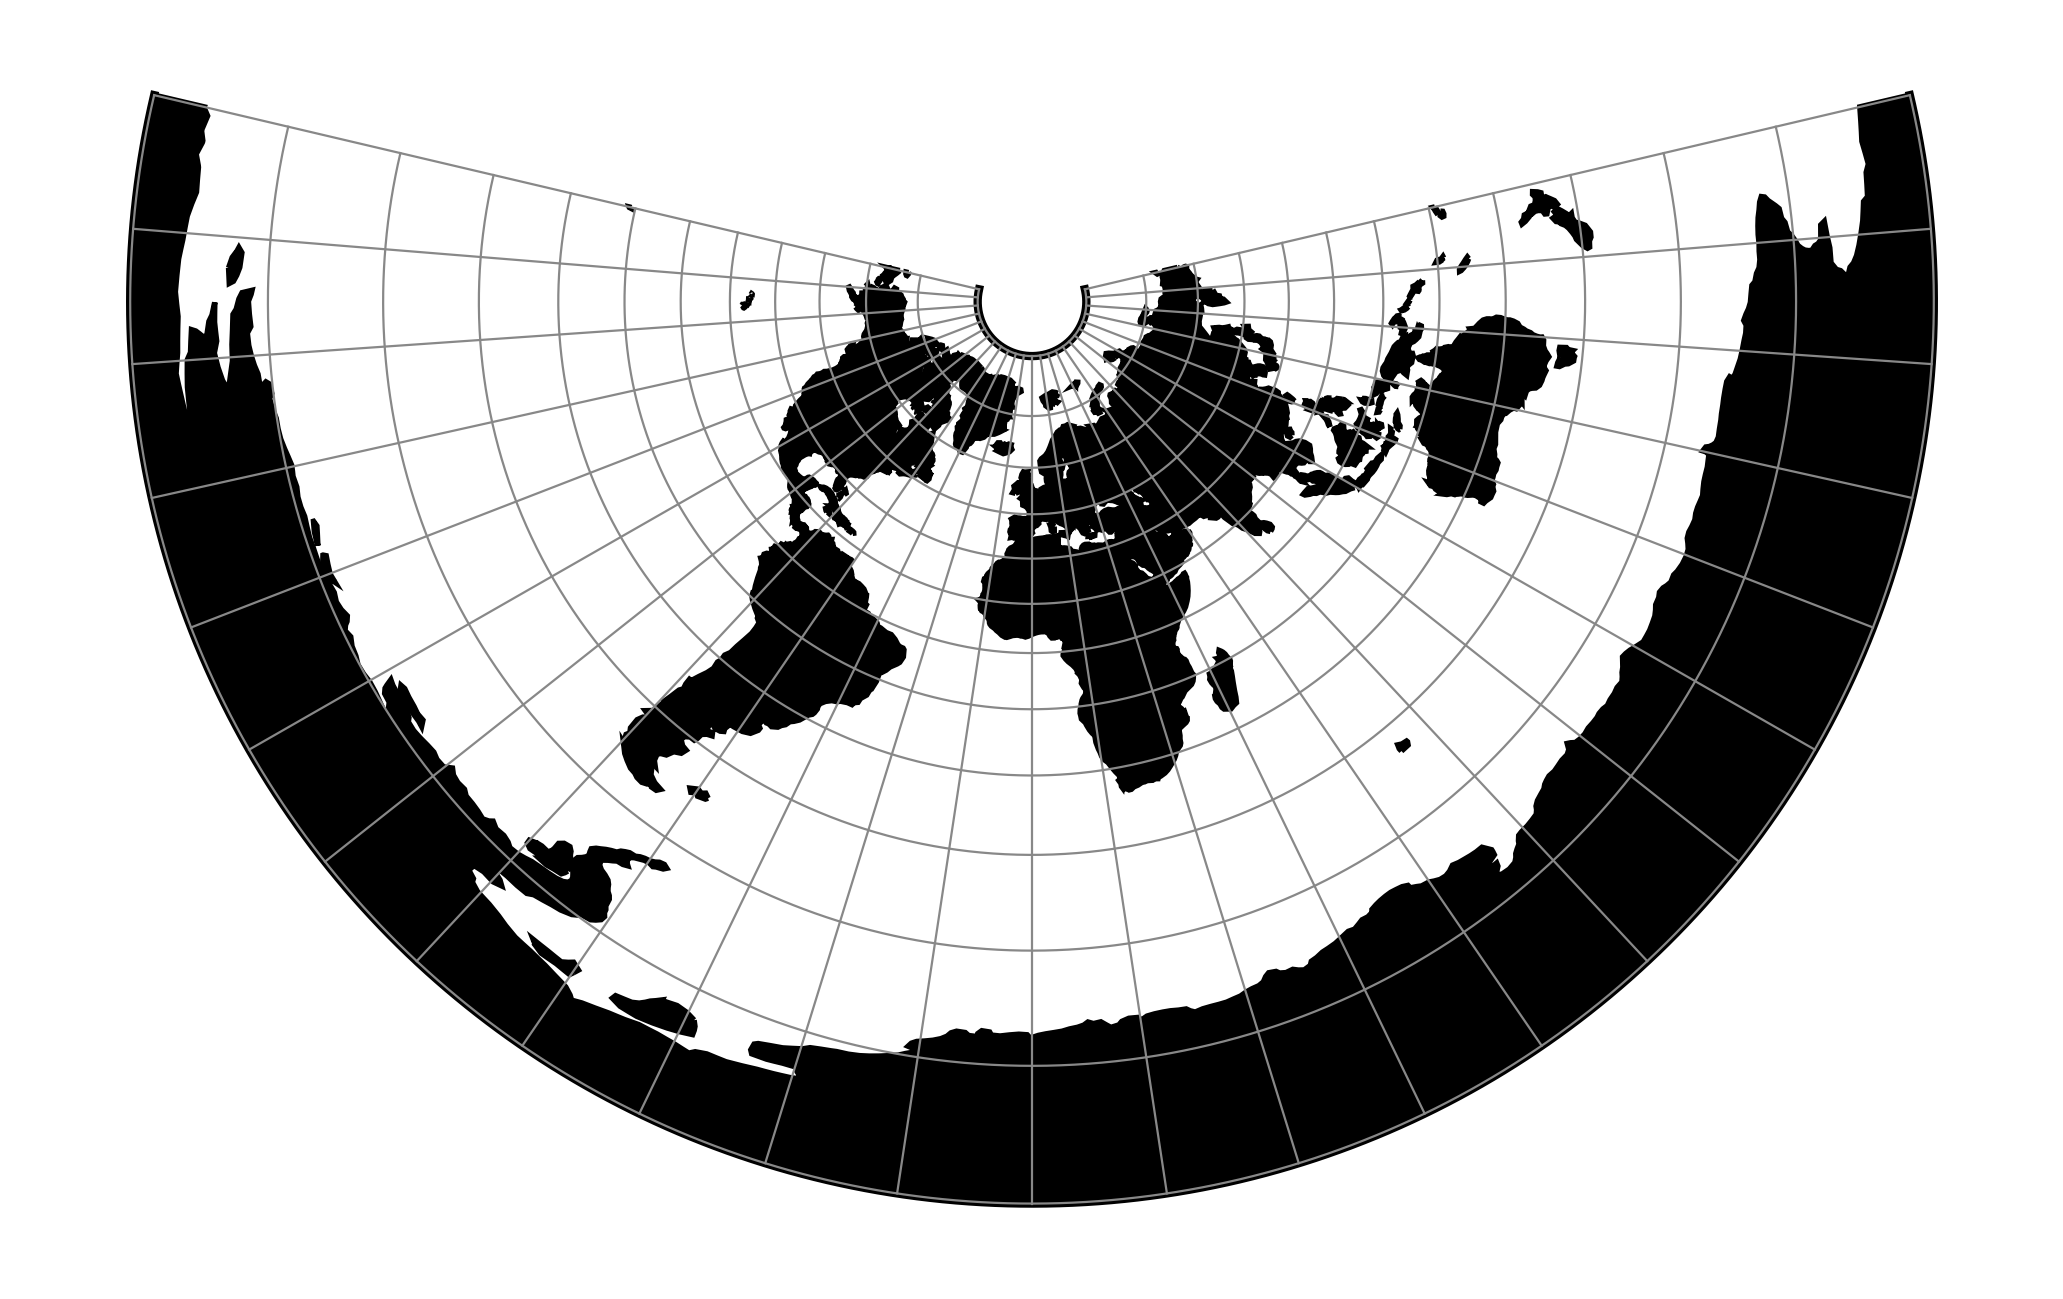
\includegraphics[width=0.9\linewidth]{figures/chapter-8/lcca.png}
        \caption{Lambert Conformal Conic Alternative (Source \cite{PROJ_SITE})}
        \label{fig:lcca_proj}
    \end{minipage}\hfill
    \begin{minipage}{0.30\textwidth}
        \centering
        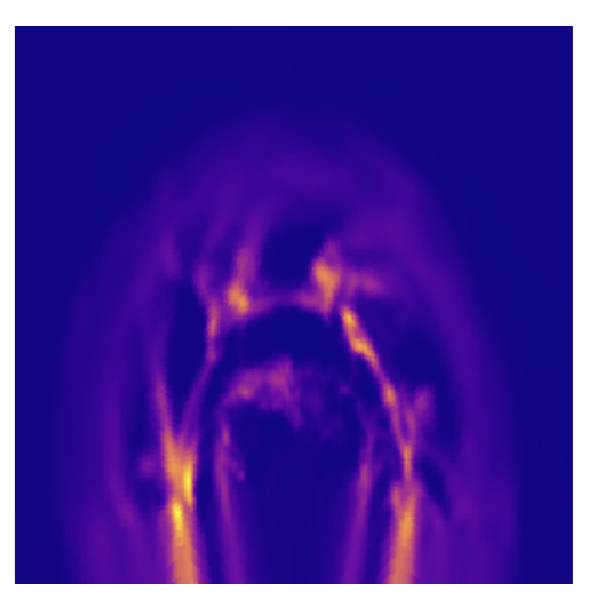
\includegraphics[width=0.9\linewidth]{figures/chapter-8/prect_lcca.png}
        \caption{Precipitation raster data as Lambert Conformal Conic Alternative projected}
        \label{fig:lcca_prect_raster}
    \end{minipage}\hfill
\end{figure}

\subsection{Results}
\begin{table}[ht]
    \centering
    \caption{Summary of Model Performance}
    \label{conic_results_table}
    \renewcommand{\arraystretch}{1.2} % Adjusts the row height
    \begin{tabular}{|l|c|c|c|c|c|}
        \hline
        \rowcolor[gray]{0.9}
        \textbf{\emph{Project Name}} & \textbf{\emph{\# Epochs}} & \textbf{\emph{MAE}} & \textbf{\emph{Validation MAE}} & \textbf{\emph{MAPE}} & \textbf{\emph{Validation MAPE}} \\ \hline
        Project 1                    & 50                        & 0.05                & 0.06                           & 5\%                  & 6\%                             \\ \hline
        Project 2                    & 30                        & 0.04                & 0.05                           & 4\%                  & 5\%                             \\ \hline
        Project 3                    & 100                       & 0.03                & 0.04                           & 3\%                  & 4\%                             \\ \hline
    \end{tabular}
\end{table}